\section{Fish Grasping Simulation}\label{sec:simulation}

Supervised learning techniques requires a substantial amount of data to learn generalised functions for utilisation on unseen examples in any environment. The rate at which we can acquire such data in the our universe is limited by time and physical constants of the universe we live in, furthermore this form of acquisition may also be costly financially. We can circumvent these limitations by carrying out precise simulations emulating the physical properties of our universe. The precision of the simulation is key when any model trained on the simulated data, is applied on the data from the true distribution %$p_{data}(X)$
the simulation was trying to emulate. 
%This shift in the input data distribution is coined domain transfer, in that the model is utilised in another domain than it was trained in. 
Failure to achieve sufficient precision in the simulations will most likely unexpected and unwanted behaviour by the agent using the model due significant change in distribution of the input and the model being slightly overfit to noise in the synthetically generated dataset.

Having the ability to control and observe every parameter in a simulation environment means that we can certainty rely on the observed state of the environment. This eases the development of domain specific and somewhat intelligent programs that carry perfectly carry out a intended task, this allows any observer to try learn from experts with fully observable state and seek out important cues that help with the task at hand.   

With importance of transferability of model's domain in mind we should sought to make a simulation as precise as is computationally feasible.

\cite{Dyrstad2016} constructed such simulations to allow models to learn how to detect and grasp objects in an environments but not to navigate the environment or approach grasp position and orientation. The contribution of the constructed simulation environment is to enable compilation of data set that enable machine learning models to learn programs from some scripted behaviour in simulated environments, the focus on realism of the simulation then enables models, post-training, to be applied in our universe.

Screenshots from the simulation in action can be seen in appendix~\ref{app:simulation}.

\subsection{States}\label{sec:states}

The scripted behaviour is implemented with state machines, observing and registering events in the environment and then acting accordingly.

\begin{figure}
\centering
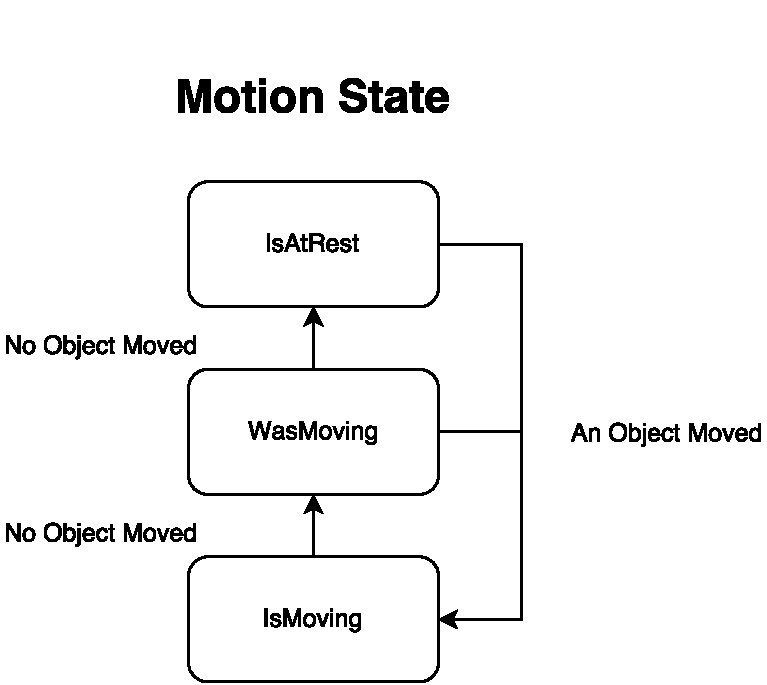
\includegraphics[width=.4\linewidth]{figures/statediagrams/motion-states.pdf}
\caption{motion-states}
\label{fig:motion-states}
\end{figure}

We want to know whether the current path we are following, is still valid or a collision might be occurring with an obstuction on the current course. Should it be the case that is not valid anymore, then we would want to recalculate and plan a new collision free course for the newly changed environment. The state machine depicted in fig.~\ref{fig:motion-states} is responsible for keeping track of this.

Similarly when a possible target object changes its orientation or location/position in the environment, we would want to recalculate the path and valid grasp or possibly even reconsider which target to pick up. It is implemented using the same state machine as depicted in fig.~\ref{fig:motion-states} but is tracking target instead of obstructions in the environment.

We could recalculate the target object and path on every frame, but as some noticeable time may sometimes be spend calculating such path in a difficult environment, we only want to recalculate when the environment changes and it is necessary.

\begin{figure}
\centering
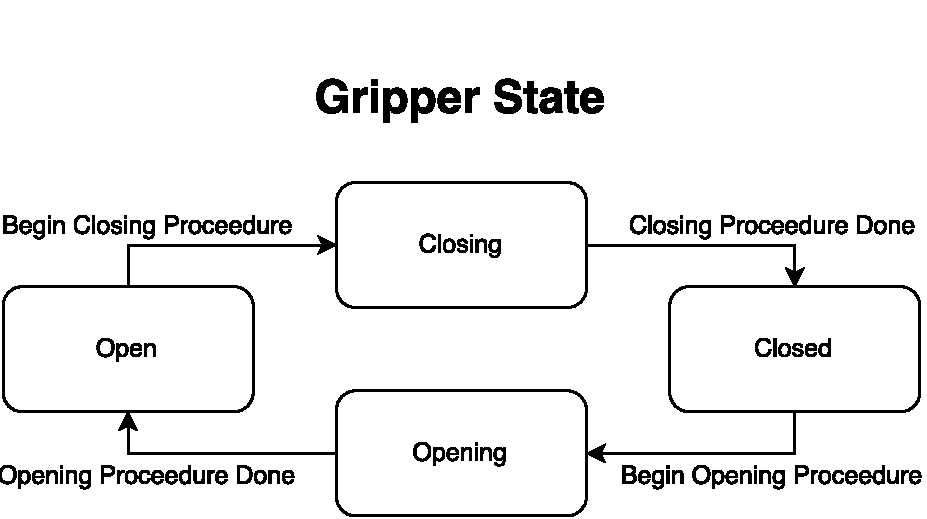
\includegraphics[width=.6\linewidth]{figures/statediagrams/gripper.pdf}
\caption{gripper}
\label{fig:gripper}
\end{figure}

Throughout the simulation we would want to track whether the grippers claw is in an open or closed position. Note that the simulation runs in discrete time steps which means that the gripper can be closing to reach a closed state or opening to an open state, leading to the gripper having 4 possible states, open, opening, closed and closing. Another way to track this was with a percentage but because the closed state position is not a fixed but in fact is dependent on the orientation, position and size of the target object the gripper is picking up, then a simpler two static state solution was chosen, depicted in fig.~\ref{fig:gripper}.

\begin{figure}
\centering
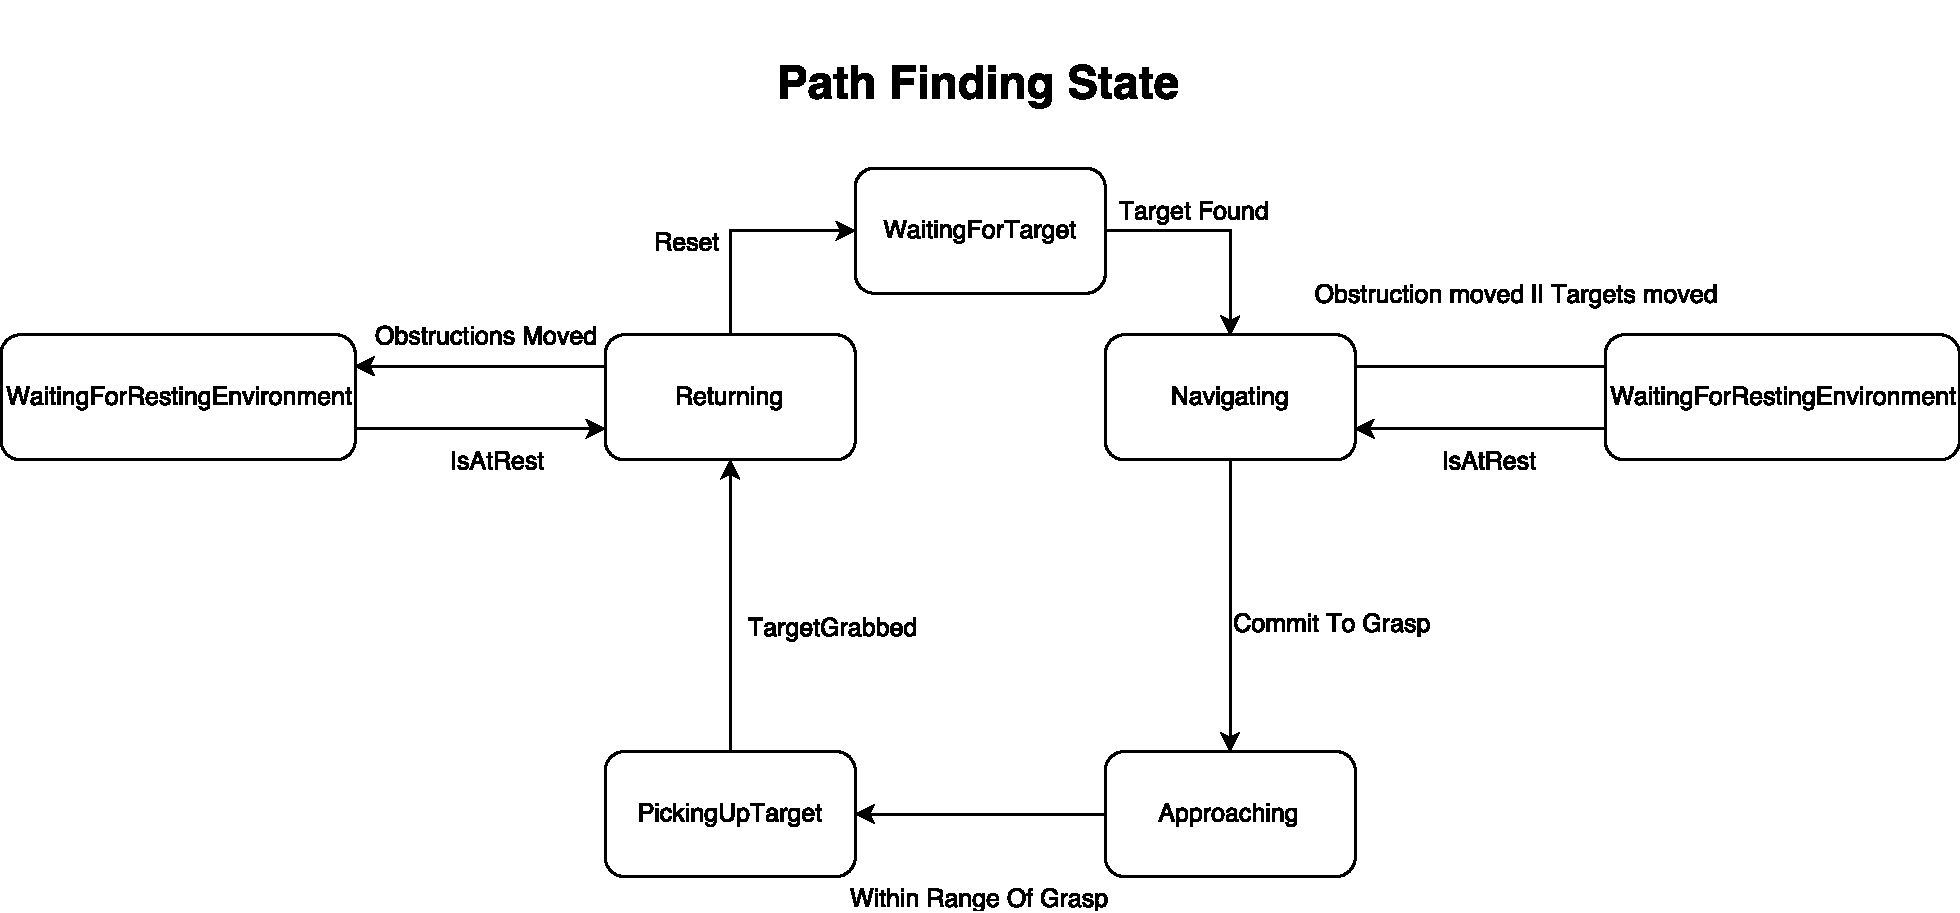
\includegraphics[width=\linewidth]{figures/statediagrams/path.pdf}
\caption{path}
\label{fig:path}
\end{figure}

Along the planned path the gripper is following, the gripper transitions through a number of phases that changes its behaviour slightly, like not rotating according to the targets orientation anymore or waiting for the environment to be at rest before continuing. fig.~\ref{fig:path} shows these states or phases if you will.

\begin{figure}
\centering
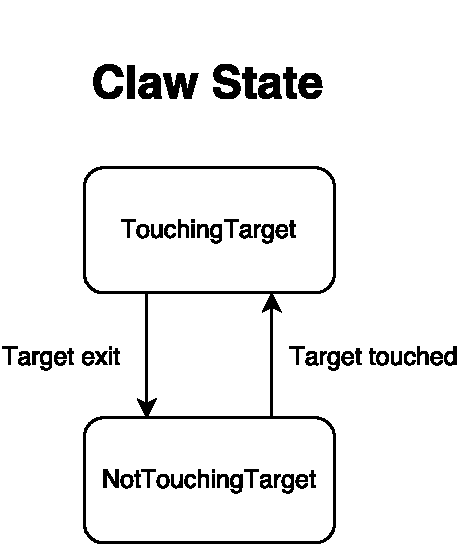
\includegraphics[width=.3\linewidth]{figures/statediagrams/claw-states.pdf}
\caption{claw states}
\label{fig:claw}
\end{figure}

Both claws of the gripper can possibly interacting the target, by touching it and thereby also be able to affect the target's position and orientation. The two states for each claw help to indicate whether or not we belief that we have a secure grasp around the object we are picking up. If the target is only touching one claw it is possible that the object, in this case fish, will just slip out of the gripper during pick up procedure or return procedure, fig.~\ref{fig:claw} depicts the states for these claws.

\begin{figure}
\centering
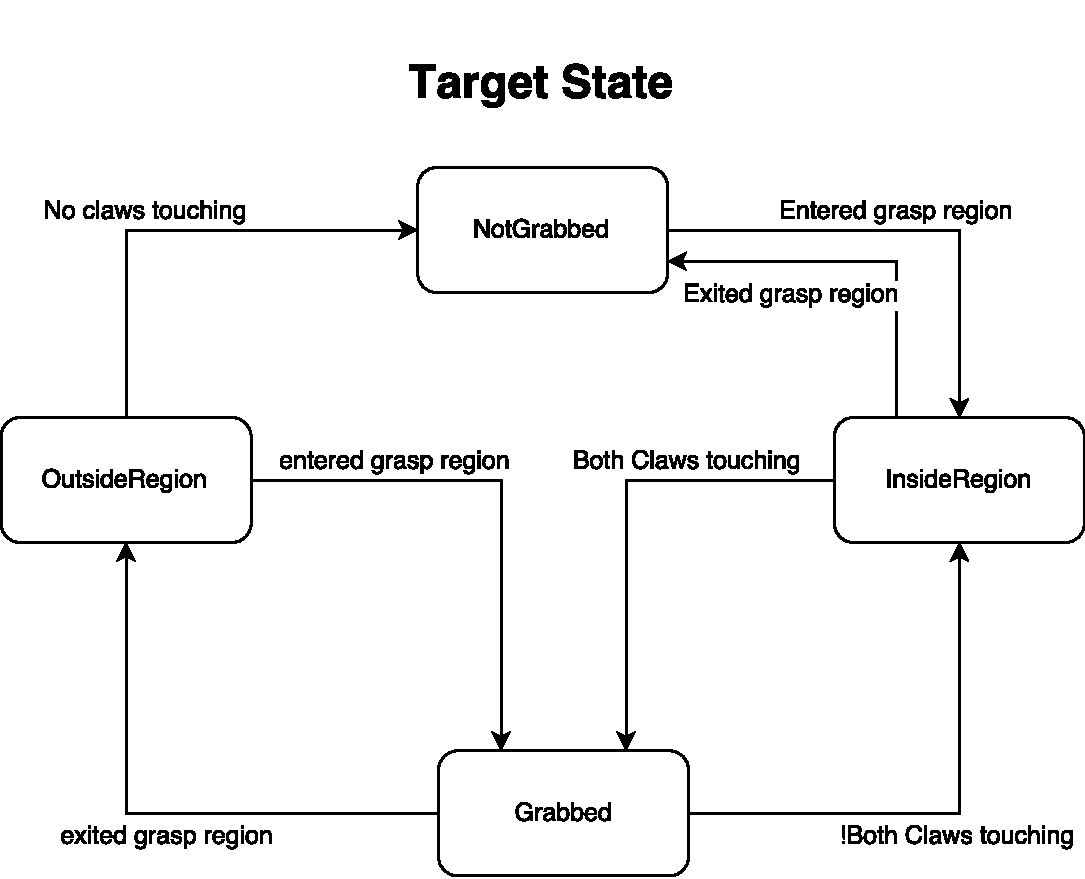
\includegraphics[width=.8\linewidth]{figures/statediagrams/target.pdf}
\caption{target}
\label{fig:target}
\end{figure}

The state machine depicted in fig.~\ref{fig:target}, tries to capture our current belief of the state of the target being picked up, it is possible that we lose the target during travel to destination or that we fail to pick it up in the first place. When picking up the target we are tracking whether the target is inside the region of the gripper where we expect a secure grasp, when this is the case we can change the state of the gripper to closing, which in turns closes claws and secures the target in place in the gripper.

%\subsection{Usage Guide}

This section will briefly describe how to use the neodroid simulation.

The source code for the simulation environment is hosted at \url{https://github.com/sintefneodroid/simulation}.

\subsection{Issues}

The environment has some issues that degrades the realism of the simulation. 

\subsubsection{Shadows}

Calculating how each discrete point in the environment should be lighted is computationally extensive when trying to emulate how lighting in our universe behaves, surfaces can be reflexive, luminant and the might be multiple light sources. Some assumptions and short comings is required to make rendering rate fast and smooth, this leads to limitations in what level of realism, we can achieve. In \cite{unity3d} each light source has shadow map with some fixed resolution according to the quality setting and the amount available ram on the gpu \cite{unityshadowmapsize}, this means if the light map span a larger area the pixelation is the shadows projected into the scene than when the light span a smaller area but keeps the same fixed resolution. Note that is the span is both affected by the distance the light source is from the projected surface and the field the light source spans in degrees. Section ~\ref{sec:shadowsexperiment} will explorer this issue further.

\subsubsection{Friction}

As of now friction between the target and the gripper relies on \cite{unityphysics} physics system, which is imprecise at best. To keep the target relatively stable within the jaws of the gripper, the target object is applied the same forces at the gripper additional to any gravitational or velocity forces affecting the target. It is important to note that these forces would be preferred to be affecting the target indirectly through the proxy colliders on the grippers jaws, but this is not the case as the \cite{unity3d} physics system is not precise enough and simply cant approximate this intented behaviour.

\subsubsection{Colliders}

One issue with the current simulation is when the object to be picked up has more than one collider interconnected via joint, then the \cite{unityphysics} physics system ends up in a unstable simulation and causes quite unpredictable and nonsensical undesired behaviour, the individual colliders of the fish-like object chaotically collides with the gripper while constantly trying the keep up the maximum angle of the joints until twisting the object out the grasp of the gripper.

The source code for the simulation environment is hosted at \url{https://github.com/sintefneodroid/simulation}.